\section{Einarbeitung}
In der Einarbeitungsphase haben wir uns zunächst für eine Hadoop-Arbeitsumgebung entschieden. Da die meisten Projektteilnehmer über lediglich vier Gigabyte Arbeitsspeicher verfügen, fiel unsere Wahl auf die ressourcenschonende Hortonworks Sandbox \footnote{Siehe: \url{http://hortonworks.com/products/hortonworks-sandbox/}}, die bei allen Teilnehmern problemlos ausgeführt werden konnte. Unter Verwendung der Sandbox haben wir den Umgang mit dem Hadoop-Ecosystem gelernt und erste Map/Reduce-Jobs ausgeführt. Darüber hinaus konnten wir weitere Tools wie Hive und Pig verwenden.

\subsection{Datenmodell}
Abbildung \ref{fig:ShoppersTables} zeigt das Datenmodell, dass aus den Entitäten transactions, history, offers, und submissions besteht...
\todo[inline]{Grafik passt nicht: trainHistory und testHistory berücksichtigen!}
\begin{figure}[h]
\centering
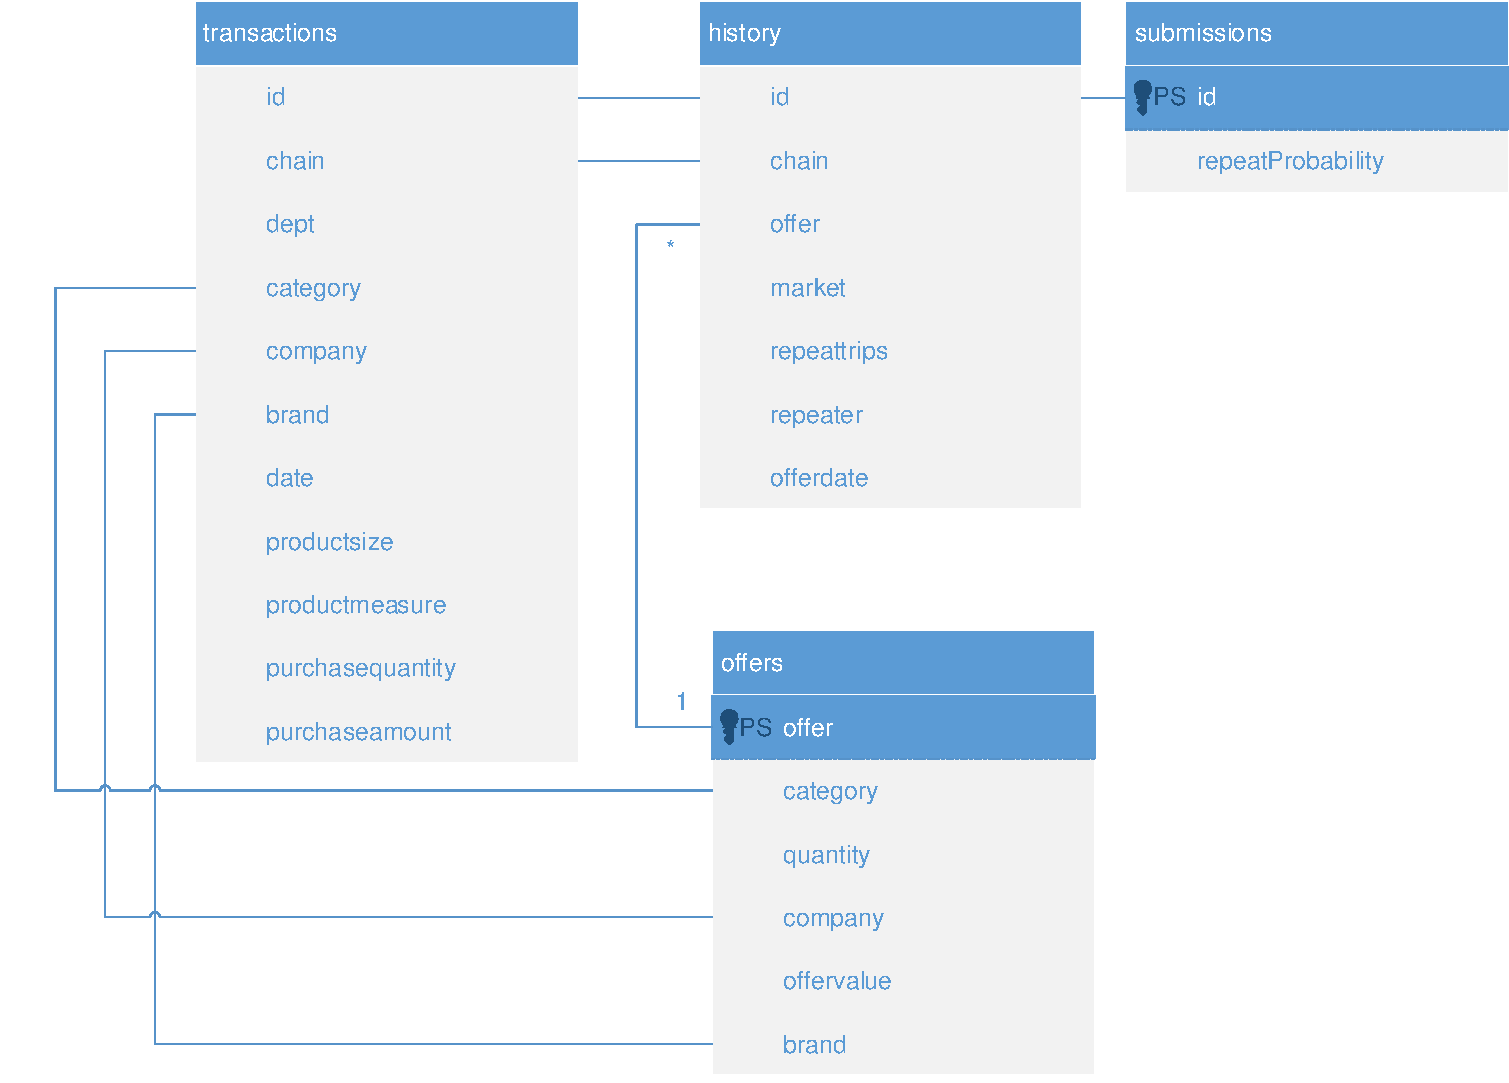
\includegraphics[width=0.7\linewidth]{Bilder/ShoppersTables}
\caption{Das Datenmodell}
\label{fig:ShoppersTables}
\end{figure}





\subsection{Data-Mining-Verfahren}

\subsection{Technologieentscheidung}

Pig vs Hive
Entscheidung für Hive aufgrund strukturierter Daten

Hive -> Features
? -> Auswertung der Features
